\documentclass[journal,12pt,twocolumn]{IEEEtran}

\usepackage{setspace}
\usepackage{gensymb}
\singlespacing
\usepackage[cmex10]{amsmath}
\usepackage{amssymb}
\usepackage{xurl}
\usepackage{tabularx}
\usepackage{amsthm}
\usepackage{comment}
\usepackage{mathrsfs}
\usepackage{txfonts}
\usepackage{stfloats}
\usepackage{bm}
\usepackage{cite}
\usepackage{cases}
\usepackage{subfig}
\usepackage{arydshln}
\usepackage{longtable}
\usepackage{multirow}

\usepackage{enumitem}
\usepackage{mathtools}
\usepackage{steinmetz}
\usepackage{tikz}
\usepackage{circuitikz}
\usepackage{verbatim}
\usepackage{tfrupee}
\usepackage[breaklinks=true]{hyperref}
\usepackage{graphicx}
\usepackage{tkz-euclide}
\usetikzlibrary{automata, positioning}
\usetikzlibrary{calc,math}
\usepackage{listings}
    \usepackage{color}                                            %%
    \usepackage{array}                                            %%
    \usepackage{longtable}                                        %%
    \usepackage{calc}                                             %%
    \usepackage{multirow}                                         %%
    \usepackage{hhline}                                           %%
    \usepackage{ifthen}                                           %%
    \usepackage{lscape}     
\usepackage{multicol}
\usepackage{chngcntr}
\usepackage{blkarray}

\DeclareMathOperator*{\Res}{Res}

\renewcommand\thesection{\arabic{section}}
\renewcommand\thesubsection{\thesection.\arabic{subsection}}
\renewcommand\thesubsubsection{\thesubsection.\arabic{subsubsection}}

\renewcommand\thesectiondis{\arabic{section}}
\renewcommand\thesubsectiondis{\thesectiondis.\arabic{subsection}}
\renewcommand\thesubsubsectiondis{\thesubsectiondis.\arabic{subsubsection}}


\hyphenation{op-tical net-works semi-conduc-tor}
\def\inputGnumericTable{}                                 %%

\lstset{
%language=C,
frame=single, 
breaklines=true,
columns=fullflexible
}
\begin{document}


\newtheorem{theorem}{Theorem}[section]
\newtheorem{problem}{Problem}
\newtheorem{proposition}{Proposition}[section]
\newtheorem{lemma}{Lemma}[section]
\newtheorem{corollary}[theorem]{Corollary}
\newtheorem{example}{Example}[section]
\newtheorem{definition}[problem]{Definition}

\newcommand{\BEQA}{\begin{eqnarray}}
\newcommand{\EEQA}{\end{eqnarray}}
\newcommand{\define}{\stackrel{\triangle}{=}}
\bibliographystyle{IEEEtran}
\raggedbottom
\setlength{\parindent}{0pt}
\providecommand{\mbf}{\mathbf}
\providecommand{\pr}[1]{\ensuremath{\Pr\left(#1\right)}}
\providecommand{\qfunc}[1]{\ensuremath{Q\left(#1\right)}}
\providecommand{\sbrak}[1]{\ensuremath{{}\left[#1\right]}}
\providecommand{\lsbrak}[1]{\ensuremath{{}\left[#1\right.}}
\providecommand{\rsbrak}[1]{\ensuremath{{}\left.#1\right]}}
\providecommand{\brak}[1]{\ensuremath{\left(#1\right)}}
\providecommand{\lbrak}[1]{\ensuremath{\left(#1\right.}}
\providecommand{\rbrak}[1]{\ensuremath{\left.#1\right)}}
\providecommand{\cbrak}[1]{\ensuremath{\left\{#1\right\}}}
\providecommand{\lcbrak}[1]{\ensuremath{\left\{#1\right.}}
\providecommand{\rcbrak}[1]{\ensuremath{\left.#1\right\}}}
\theoremstyle{remark}
\newtheorem{rem}{Remark}
\newcommand{\sgn}{\mathop{\mathrm{sgn}}}
\providecommand{\abs}[1]{\vert#1\vert}
\providecommand{\res}[1]{\Res\displaylimits_{#1}} 
\providecommand{\norm}[1]{\lVert#1\rVert}
%\providecommand{\norm}[1]{\lVert#1\rVert}
\providecommand{\mtx}[1]{\mathbf{#1}}
\providecommand{\mean}[1]{E[ #1 ]}
\providecommand{\fourier}{\overset{\mathcal{F}}{ \rightleftharpoons}}
%\providecommand{\hilbert}{\overset{\mathcal{H}}{ \rightleftharpoons}}
\providecommand{\system}{\overset{\mathcal{H}}{ \longleftrightarrow}}
	%\newcommand{\solution}[2]{\textbf{Solution:}{#1}}
\newcommand{\solution}{\noindent \textbf{Solution: }}
\newcommand{\cosec}{\,\text{cosec}\,}
\providecommand{\dec}[2]{\ensuremath{\overset{#1}{\underset{#2}{\gtrless}}}}
\newcommand{\myvec}[1]{\ensuremath{\begin{pmatrix}#1\end{pmatrix}}}
\newcommand{\mydet}[1]{\ensuremath{\begin{vmatrix}#1\end{vmatrix}}}
\newcommand*{\permcomb}[4][0mu]{{{}^{#3}\mkern#1#2_{#4}}}
\newcommand*{\perm}[1][-3mu]{\permcomb[#1]{P}}
\newcommand*{\comb}[1][-1mu]{\permcomb[#1]{C}}
\numberwithin{equation}{subsection}
\makeatletter
\@addtoreset{figure}{problem}
\makeatother
\let\StandardTheFigure\thefigure
\let\vec\mathbf
\renewcommand{\thefigure}{\theproblem}
\def\putbox#1#2#3{\makebox[0in][l]{\makebox[#1][l]{}\raisebox{\baselineskip}[0in][0in]{\raisebox{#2}[0in][0in]{#3}}}}
     \def\rightbox#1{\makebox[0in][r]{#1}}
     \def\centbox#1{\makebox[0in]{#1}}
     \def\topbox#1{\raisebox{-\baselineskip}[0in][0in]{#1}}
     \def\midbox#1{\raisebox{-0.5\baselineskip}[0in][0in]{#1}}
\vspace{3cm}
\title{Assignment 5}
\author{Tanay Yadav - AI20BTECH11026}
\maketitle
\newpage
\bigskip
\renewcommand{\thefigure}{\theenumi}
\renewcommand{\thetable}{\theenumi}
Download the python codes from: 
%
\begin{lstlisting}
https://github.com/tanayyadav28/EE3900-Assignments/blob/main/Assignment_5/code/Assignment_5.py
\end{lstlisting}
Download the latex-tikz codes from: 
%
\begin{lstlisting}
https://github.com/tanayyadav28/EE3900-Assignments/blob/main/Assignment_5/Assignment_5.tex
\end{lstlisting}
\section{Problem}
[Quadratic Forms 2.22]
Solve:
\begin{align}
    x^2 + x + 1 &= 0
\end{align}
\section{Solution}
Let
\begin{align}
    y &= x^2 + x + 1 = 0
\end{align}
Representing $y$ in vector form,
\begin{align}
    y &= \vec{x}^T\myvec{1 & 0\\0 & 0}\vec{x} + 2\myvec{\frac{1}{2} & 0}\vec{x} + 1
\end{align}
where,
\begin{align}
    \vec{x} = \myvec{x\\0}
\end{align}
Putting $y = 0$ we get,
\begin{align}
    x^2 + x + 1 &= 0\\
    x^2 + 2\left(\frac{1}{2}\right)x + \frac{1}{4} + \frac{3}{4} &= 0\\
    \left(x + \frac{1}{2}\right)^2 + \frac{3}{4} &= 0\\
    \left(x + \frac{1}{2}\right)^2 &= -\frac{3}{4}
\end{align}
A square of a real number can never be negative. \\
Therefore, the given equation has no real roots which is verified by the python plot.\\
Obtaining the Affine Transformation,
\begin{align}
    V &= \myvec{1 & 0\\ 0 & 0}\\
    \vec{u} &= \myvec{\frac{1}{2} \\ -\frac{1}{2}}\\
    \textit{f} &= 1 
\end{align}
The equation for Affine transformation is:
\begin{align}
    \vec{x} = \vec{P}\vec{y} + \vec{c}
\end{align}
The Eigenvalues of $V$ are:
\begin{align}
    \lambda_1 &= 1\\
    \lambda_2 &= 0\\
    \vec{D} &= \myvec{1 & 0\\ 0 & 0}
\end{align}
The Eigen vectors of $V$ are:
\begin{align}
    \vec{p_1} &= \myvec{0 \\ 1}\\
    \vec{p_2} &= \myvec{1 \\ 0}\\
    \therefore \vec{P} &= \myvec{\vec{p_1} & \vec{p_2}}\\
    \therefore \vec{P} &= \myvec{0 & 1\\1 & 0}
\end{align}
Since, $\mydet{V} = 0$
\begin{align}
    \myvec{\vec{u}^T + \eta\vec{p}^T_1\\V}\vec{c} &= \myvec{-f \\ \eta\vec{p_1} - \vec{u}}\\
    \eta &= \vec{u^T}\vec{p_1}\\
    \therefore \eta &= -\frac{1}{2}\\
    \myvec{\frac{1}{2} & -1\\1 & 0\\0 & 0}\vec{c} &= \myvec{-1 \\ -\frac{1}{2} \\ 0} \\
    \vec{c} &= \myvec{-\frac{1}{2}\\\frac{3}{4}}
\end{align}
The quadratic equation does not have real roots if:
\begin{align}
    (\vec{p_1}^T\vec{c})(\vec{p_2}^T\vec{V}\vec{p_2}) &> 0
\end{align}
Substituting the values,
\begin{align}
    \left(\frac{3}{4}\right)(1) &= \frac{3}{4} > 0
\end{align}
Hence, the given equation has no real roots.
\begin{figure}[h]
    \centering
    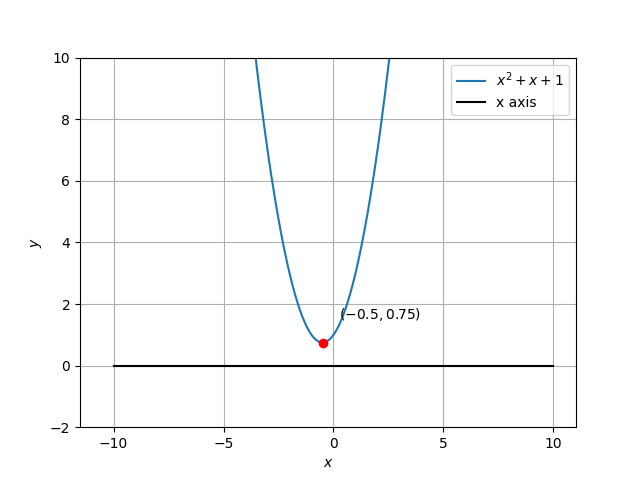
\includegraphics[scale = 0.5]{Figure_1.png}
    \caption{Plot from Python Code.}
    \label{fig:my_label}
\end{figure}


\end{document}
